\subsection{Descrizione dei soggetti reclutati e metrice adottate}

Per la presente sperimentazione sono stati definiti cinque partecipanti fittizi, creati appositamente per simulare un campione eterogeneo di utenti tipici dell’applicazione di annunci immobiliari.
I profili selezionati rappresentano diverse tipologie d’utenza, così da coprire una gamma varia di competenze tecnologiche, ruoli e obiettivi di utilizzo:

\begin{enumerate}
	
	\item \textbf{Agente immobiliare}: A questo profilo sono stati assegnati task relativi alla sezione gestionale della piattaforma, in quanto, grazie all’esperienza professionale, possiede già familiarità con strumenti digitali e sistemi di gestione di annunci.
	
	\item \textbf{Giovane cercatore}: Si tratta di uno studente o giovane lavoratore che si approccia per la prima volta al dominio immobiliare. Utilizza prevalentemente il dispositivo mobile e ha una buona abilità generale nella navigazione web, ma scarsa esperienza con servizi di annunci. L’esperimento su questo profilo è utile per valutare l’intuitività e l’usabilità del sistema da parte di utenti alle prime esperienze.
	
	
	\item \textbf{Adulto con esigenze familiari}: Questo utente ha una buona conoscenza del dominio immobiliare e dimestichezza media con la tecnologia. È in grado di comprendere termini specifici come “mutuo”, “contratto” o “numero di locali”. Gli vengono assegnati task leggermente più complessi, per verificare l’efficacia del sistema in scenari d’uso realistici e articolati.
	
	\item \textbf{Utente anziano}: Gli utenti appartenenti a questa fascia d’età (oltre i 60 anni) tendono ad avere minore familiarità con la navigazione web. Sono quindi assegnati task semplici, come la ricerca di un annuncio in una determinata zona o l’individuazione di un contatto telefonico, simulando, ad esempio, una madre che aiuta la figlia a trovare casa. Questo profilo è utile per valutare la chiarezza dell’interfaccia e la leggibilità delle informazioni.
	
	\item \textbf{Proprietario di agenzia immobiliare}: Simile al profilo dell’agente, ma con una visione gestionale più ampia. Si presume una buona competenza tecnologica e la necessità di monitorare più annunci e collaboratori. I task assegnati riguardano funzioni di controllo e gestione multipla.
	
\end{enumerate}

Di seguito viene riportata una tabella riassuntiva che descrive gli utenti reclutati e i task specifici assegnati.

\begin{figure}[H]
	\centering
	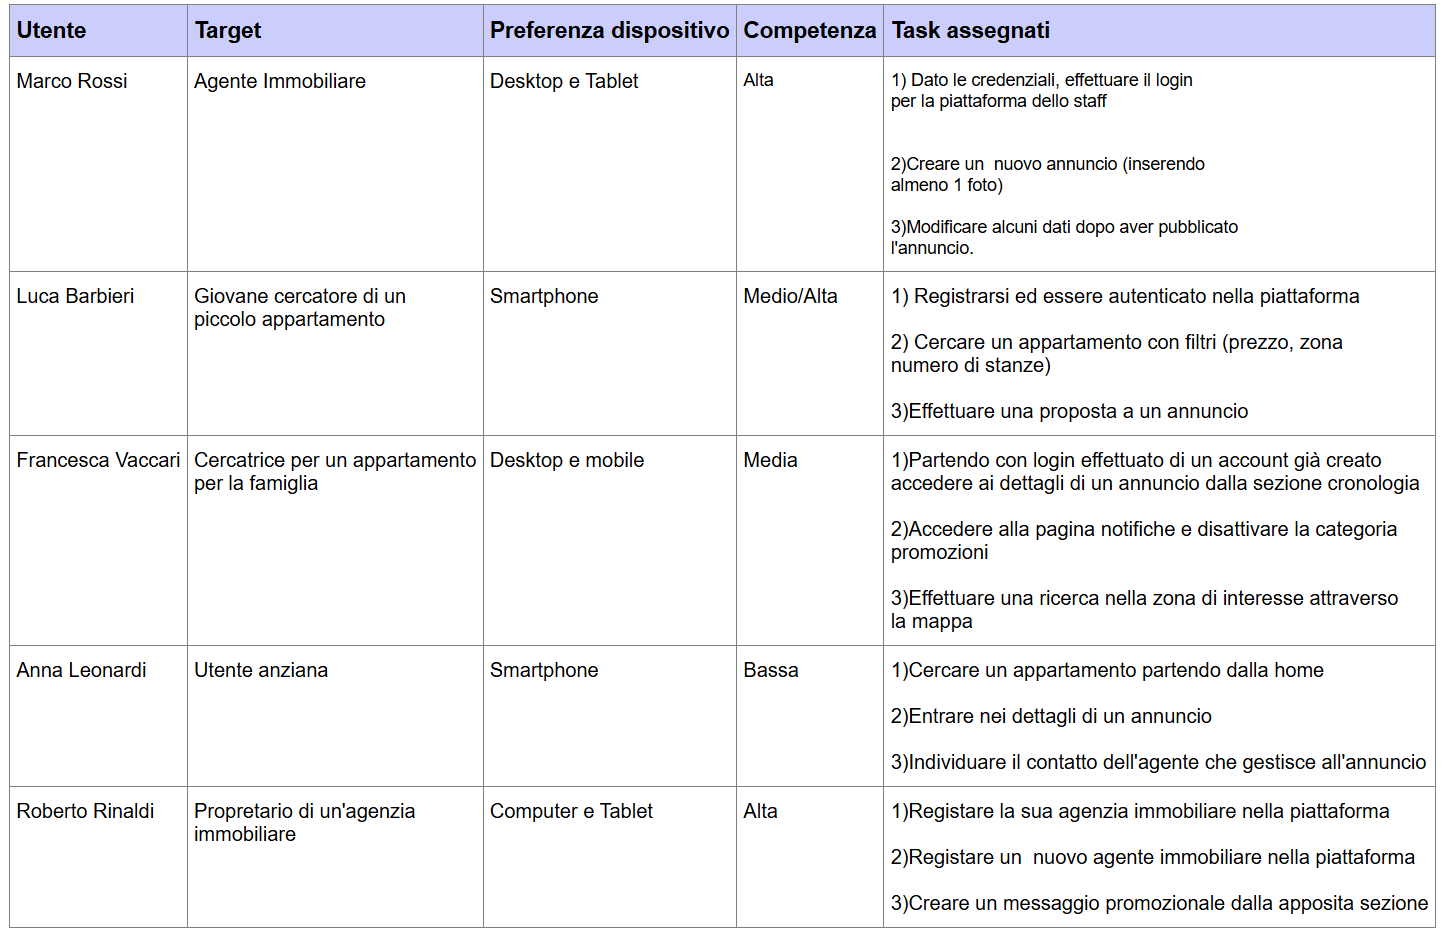
\includegraphics[width=\linewidth]{Immagini/esperimento finale/tabella utenti.png}
	\caption[tabella utenti]{Tabella utenti reclutati nell'esperimento}
\end{figure}

A ciascun partecipante sono stati proposti tre task principali inerenti alla loro categoria. Dopo l'osservazione degli esperimenti sono state adottate le seguenti metriche:

\vspace{0.5cm} % Aggiunge spazio prima della sezione

\textbf{1. Tempo medio per completare un Task}
\begin{equation}
	T_{\text{medio}} = \frac{\sum_{i=1}^{n} T_i}{n}
\end{equation}
dove \( T_i \) è il tempo impiegato dall'utente \( i \) per completare il task e \( n \) è il numero totale di utenti.

\vspace{0.5cm} % Aggiunge spazio prima della sezione
\textbf{2. Tasso di completamento di un Task}
\begin{equation}
	T_{\text{completamento}} = \frac{U_{\text{completati}}}{U_{\text{totali}}} \times 100
\end{equation}
dove \( U_{\text{completati}} \) è il numero di utenti che hanno completato il task e \( U_{\text{totali}} \) è il numero totale di utenti che hanno provato il task.

\vspace{0.5cm} % Aggiunge spazio prima della sezione
\textbf{3. Errore Medio per Task}
\begin{equation}
	E_{\text{medio}} = \frac{\sum_{i=1}^{n} E_i}{n}
\end{equation}
dove \( E_i \) è il numero di errori commessi dall'utente \( i \) durante il task.

\vspace{0.5cm} % Aggiunge spazio prima della sezione
\textbf{4. Customer Satisfaction Score}
\begin{equation}
	CSAT = \frac{\sum_{i=1}^{n} S_i}{n} \times 100
\end{equation}
dove \( S_i \) è il punteggio di soddisfazione dato dall'utente \( i \) e \( n \) è il numero totale di risposte raccolte.

\vspace{0.5cm} % Aggiunge spazio prima della sezione
\textbf{5. System Usability Scale (SUS)}
\newline
\newline
Il \textbf{System Usability Scale (SUS)} è un metodo standardizzato, introdotto da \textbf{John Brooke} nel 1986, utilizzato per misurare l’usabilità di un prodotto attraverso un questionario composto da \textbf{10 affermazioni}. Gli utenti rispondono utilizzando una \textbf{scala Likert a 5 punti}, esprimendo il loro grado di accordo o disaccordo. Il punteggio complessivo, che varia da 0 a 100, fornisce una misura quantitativa dell’usabilità percepita, consentendo di confrontare i risultati con benchmark consolidati.
\vspace{0.5cm} % Aggiunge spazio prima della sezione

Per ogni utente è stato realizzato un questionario apposito inerente ai task completati. Di seguito presentiamo i 5 questionari sottoposti agli utenti.

\vspace{0.5cm} % Aggiunge spazio prima della sezione
\subsubsection*{Questionario per Marco Rossi (Target: agente immobiliare)}
\vspace{0.5cm} % Aggiunge spazio prima della sezione
\begin{enumerate}
	\item \textbf{La compilazione dei campi divisi in step ha reso il processo di creazione più intuitivo e meno stancante.}
	\newline
	\texttt{Scopo}: Verificare se la suddivisione del form in più passaggi migliora l’esperienza utente, evitando un sovraccarico cognitivo e rendendo la compilazione più fluida.
	
	\item \textbf{Il bottone “Avanti” è posizionato in modo poco visibile e difficile da individuare.}
	\newline
	\texttt{Scopo}: Valutare la visibilità e l’intuitività del pulsante che consente di procedere nella compilazione, elemento essenziale per garantire una navigazione chiara e senza interruzioni.
	
	\item \textbf{I campi a scelta (non liberi) mi hanno aiutato a capire meglio il tipo di informazioni richieste e a velocizzare la compilazione.}
	\newline
	\texttt{Scopo}: Analizzare se l’uso di menu a tendina o opzioni predefinite aiuta a ridurre incertezze, errori e tempi di compilazione rispetto ai campi di testo libero.
	
	
	\item \textbf{Il numero di campi richiesti è eccessivo o insufficiente, rendendo il form poco bilanciato.}
	\newline
	\texttt{Scopo}: Ottenere un feedback sulla quantità di informazioni richieste, bilanciando completezza e semplicità d’uso, evitando di rendere il processo troppo lungo o complesso.
	
	\item \textbf{I colori utilizzati sono gradevoli e non affaticano la lettura.}
	\newline
	\texttt{Scopo}: Valutare se la combinazione di colori scelta favorisce una buona leggibilità e un’esperienza visiva piacevole, senza creare affaticamento visivo.
	
	\item \textbf{L’importazione e la gestione delle foto dell’annuncio risultano poco intuitive.}
	\newline
	\texttt{Scopo}: esaminare la semplicità e l’efficacia del meccanismo di caricamento delle immagini, una funzionalità chiave nella creazione di annunci immobiliari.
	
	\item \textbf{Trovo utile l’anteprima dell’annuncio prima di confermare la pubblicazione.}
	\newline
	\texttt{Scopo}: Capire se l’anteprima fornisce valore aggiunto agli utenti, permettendo loro di controllare e correggere eventuali errori prima della pubblicazione definitiva.
	
	\item \textbf{Non è stato intuitivo trovare dove modificare l’annuncio appena creato.}
	\newline
	\texttt{Scopo}: Testare la navigabilità del pannello e la riconoscibilità dell’icona di modifica.
	
	\item \textbf{In caso di errore (compilazione errata o parziale), i messaggi di errore sono posizionati bene e mi aiutano a capire rapidamente dove ho sbagliato.}
	\newline
	\texttt{Scopo}: Valutare la chiarezza dei messaggi di errore e il loro posizionamento, per garantire che l’utente possa correggere facilmente eventuali problemi.
	
	\item \textbf{Nel complesso, non sono soddisfatto dell’esperienza nel portare a termine i compiti assegnati.}
	\newline
	\texttt{Scopo}: Raccogliere un’indicazione generale sul livello di soddisfazione dell’utente rispetto all’intero processo, fornendo una misura qualitativa dell’usabilità percepita.
	
\end{enumerate}

\vspace{0.5cm} % Aggiunge spazio prima della sezione
\subsubsection*{Questionario per Luca Barbieri (Target: giovane cercatore)}
\vspace{0.5cm} % Aggiunge spazio prima della sezione

\begin{enumerate}
	\item \textbf{Il processo di registrazione e autenticazione risulta coerente con quello della maggior parte dei sistemi web utilizzati.}
	\newline
	\texttt{Scopo}: Verificare la coerenza esterna del sistema di registrazione e autenticazione rispetto agli standard comuni. Questa euristica di Nielsen-Molich contribuisce a ridurre il divario tra valutazione ed esecuzione, migliorando la prevedibilità del sistema.
	
	\item \textbf{La pagina dei risultati di ricerca su dispositivo mobile risulta poco pratica: i testi sono piccoli e gli elementi troppo ravvicinati.}
	\newline
	\texttt{Scopo}: Valutare la responsività e l’accessibilità dell’interfaccia su schermi ridotti, garantendo una corretta leggibilità e un adeguato spazio di interazione per il tocco.
	
	\item \textbf{Le anteprime degli annunci nella pagina dei risultati contengono informazioni utili e permettono una prima valutazione senza aprire il dettaglio.}
	\newline
	\texttt{Scopo}:Verificare l’equilibrio informativo e la chiarezza visiva delle card annuncio. L’obiettivo è garantire che testi e icone supportino la scansione cognitiva senza generare sovraccarico informativo o, al contrario, eccessiva sintesi.
	
	\item \textbf{Le parole utilizzate nei filtri di ricerca sono troppo tecniche e difficili da comprendere.}
	\newline
	\texttt{Scopo}: Assicurare la conformità al principio del linguaggio dell’utente, evitando termini di dominio specialistico non familiari. Ciò riduce il carico cognitivo e migliora la comprensibilità semantica dei filtri.
	
	\item \textbf{Riesco a comprendere chiaramente che i risultati di ricerca corrispondono ai filtri selezionati.}
	\newline
	\texttt{Scopo}: Testare la visibilità dello stato del sistema e la trasparenza dell’interazione, accertando che l’utente percepisca la consistenza tra input (filtri) e output (risultati).
	
	\item \textbf{Gli elementi presenti nella barra dei filtri risultano difficili da capire e da utilizzare correttamente.}
	\newline
	\texttt{Scopo}: Valutare l’efficacia delle affordance percettive e delle segnalazioni visive (etichette, icone, layout) nel guidare l’utente all’interazione corretta con i componenti della barra di ricerca.
	
	\item \textbf{È stato facile trovare la sezione dedicata all’invio di una proposta per un annuncio.}
	\newline
	\texttt{Scopo}: Analizzare la facilità di navigazione e la struttura informativa del sito, verificando la findability delle funzionalità più rilevanti per l’utente.
	
	\item \textbf{I campi del form per inviare una proposta non sono chiari e le descrizioni non aiutano a capire cosa inserire.}
	\newline
	\texttt{Scopo}: Misurare il carico cognitivo legato alla compilazione dei moduli e verificare la presenza di etichettature efficaci e messaggi di aiuto (principio di error prevention).
	
	\item \textbf{Dopo l’invio della proposta ho ricevuto un chiaro feedback che mi ha confermato l’avvenuta operazione.}
	\newline
	\texttt{Scopo}: Verificare l’applicazione del principio di visibilità dello stato del sistema, garantendo che l’utente percepisca la conclusione e l’esito dell’azione senza incertezza.
	
	\item \textbf{Nel complesso, non sono soddisfatto dell’esperienza nel portare a termine i compiti assegnati.}
	\newline
	\texttt{Scopo}: Raccogliere una valutazione complessiva sull’usabilità percepita, utile a integrare i dati quantitativi con una misura qualitativa di soddisfazione soggettiva.
	
\end{enumerate}

\vspace{0.5cm} % Aggiunge spazio prima della sezione
\subsubsection*{Questionario per Francesca Vaccari (Target: madre con esigenze familiari)}
\vspace{0.5cm} % Aggiunge spazio prima della sezione

\begin{enumerate}
	
	\item \textbf{Trovo pratico che la sezione dello storico delle ricerche si apra come finestra anziché come pagina dedicata.}
	\newline
	\texttt{Scopo}: Valutare se tale scelta progettuale rispetti il principio di efficienza e flessibilità d’uso, riducendo i tempi di navigazione e migliorando la continuità dell’esperienza.
	
	\item \textbf{I campi informativi presenti nello storico delle ricerche non mi aiutano a ricordare chiaramente il tipo di ricerca effettuata.}
	\newline
	\texttt{Scopo}: Verificare che il sistema favorisca il riconoscimento piuttosto che il ricordo, minimizzando il carico cognitivo a breve termine e migliorando la comprensibilità dei dati salvati.
	
	\item \textbf{Riesco a navigare nello storico delle ricerche in modo semplice anche da dispositivo mobile}
	\newline
	\texttt{Scopo}: Valutare la responsività e l’accessibilità dell’interfaccia su schermi ridotti, garantendo leggibilità, coerenza del layout e un adeguato spazio di interazione touch.
	
	\item \textbf{Faccio fatica a capire in quale categoria di notifiche mi trovo all’interno della pagina notifiche.}
	\newline
	\texttt{Scopo}: Verificare la chiarezza informativa e la visibilità della struttura gerarchica, accertando che elementi come titoli e intestazioni guidino efficacemente l’orientamento dell’utente.
	
	\item \textbf{Sono riuscita a disattivare facilmente la categoria “Promozioni” e il sistema mi ha fornito un chiaro riscontro dell’azione effettuata.}
	\newline
	\texttt{Scopo}: Testare il principio di visibilità dello stato del sistema, assicurando che l’utente riceva feedback immediati e comprensibili sulle operazioni completate.
	
	\item \textbf{Trovo che sia facile disattivare una categoria di notifica in modo involontario.}
	\newline
	\texttt{Scopo}: Valutare il principio di controllo e libertà dell’utente, verificando la presenza di meccanismi di conferma o annullamento per prevenire azioni indesiderate.
	
	\item \textbf{Trovo semplice selezionare un’area geografica durante la ricerca di immobili sulla mappa.}
	\newline
	\texttt{Scopo}: Valutare la facilità d’uso e l’intuitività della componente di mappatura, analizzando la qualità delle affordance visive (pulsanti, strumenti di disegno, zoom, ecc.).
	
	\item \textbf{Ho avuto difficoltà a capire se i risultati mostrati sulla mappa corrispondono effettivamente alla zona selezionata.}
	\newline
	\texttt{Scopo}: Testare la visibilità dello stato del sistema e la trasparenza dell’interazione, verificando la coerenza tra input (area selezionata) e output (risultati visualizzati).
	
	\item \textbf{Durante ricerche successive sulla mappa, riesco facilmente a capire se il sistema mi mostra nuovi risultati rispetto alla ricerca precedente.}
	\newline
	\texttt{Scopo}: Valutare la chiarezza dei feedback dinamici del sistema, ad esempio la presenza di indicatori di caricamento o messaggi di aggiornamento che riducono l’incertezza operativa.
	
	\item \textbf{Nel complesso, non sono soddisfatto dell’esperienza nel portare a termine i compiti assegnati.}
	\newline
	\texttt{Scopo}: Raccogliere una valutazione complessiva sull’usabilità percepita, utile a integrare i dati quantitativi con una misura qualitativa di soddisfazione soggettiva.
	
\end{enumerate}

\vspace{0.5cm} % Aggiunge spazio prima della sezione
\subsubsection*{Questionario per Anna Leonardi (Target: utente anziano)}
\vspace{0.5cm} % Aggiunge spazio prima della sezione

\begin{enumerate}
	
	\item \textbf{Ho trovato semplice il modo in cui cercare gli annunci.}
	\newline
	\texttt{Scopo}:Valutare se il sistema è intuitivo e garantisce un’adeguata usabilità anche per utenti con minore esperienza digitale, minimizzando il carico cognitivo.
	
	\item \textbf{I risultati degli annunci non erano chiari: ho avuto difficoltà a capire se fossero effettivamente inerenti alla mia ricerca.}
	\newline
	\texttt{Scopo}: Verificare che il sistema comunichi in modo chiaro lo stato corrente e la coerenza tra input e output, riducendo possibili ambiguità interpretative.
	
	\item \textbf{Testi, descrizioni e icone nei risultati erano ben leggibili e i colori non risultavano fastidiosi.}
	\newline
	\texttt{Scopo}: Valutare l’accessibilità visiva dell’interfaccia, assicurando un contrasto cromatico adeguato e uno stile grafico confortevole per utenti con ridotte capacità visive.
	
	\item \textbf{Ho avuto difficoltà ad accedere ai dettagli di un annuncio che mi interessava.}
	\newline
	\texttt{Scopo}: Verificare la corrispondenza tra il sistema e il mondo reale, assicurandosi che i percorsi d’azione siano chiari, coerenti e prevedibili anche per utenti poco esperti.
	
	\item \textbf{Ho trovato utile la presenza di una breve descrizione sopra ogni foto dell’immobile.}
	\newline
	\texttt{Scopo}:Valutare la quantità e pertinenza delle informazioni presentate, garantendo un equilibrio tra completezza e semplicità di comprensione.
	
	\item \textbf{Ho trovato confusa la pagina dei dettagli di un annuncio.}
	\newline
	\texttt{Scopo}: Analizzare la struttura informativa e il layout visivo, individuando eventuali problemi di organizzazione spaziale o di eccessiva densità informativa.
	
	\item \textbf{Ho trovato facilmente la sezione relativa all’autore dell’annuncio.}
	\newline
	\texttt{Scopo}: Valutare la findability e il posizionamento della sezione dedicata all’agente, assicurandosi che sia facilmente individuabile anche per utenti con poca familiarità con le interfacce web.
	
	\item \textbf{La sezione dedicata agli agenti contiene poche informazioni.}
	\newline
	\texttt{Scopo}: Valutare l’adeguatezza informativa e identificare la necessità di integrare dati aggiuntivi per migliorare la fiducia e la chiarezza dell’interazione.
	
	\item \textbf{Trovo molto utile la presenza di una sezione dedicata all’autore dell’annuncio, che mi permetta di contattarlo anche al di fuori del sistema.}
	\newline
	\texttt{Scopo}:Valutare il grado di accessibilità funzionale, offrendo alternative di contatto (es. telefono, email) per ridurre la complessità operativa legata ai sistemi interni di messaggistica.
	
	\item \textbf{Nel complesso, non sono soddisfatto dell’esperienza nel portare a termine i compiti assegnati.}
	\newline
	\texttt{Scopo}: Raccogliere una valutazione complessiva sull’usabilità percepita, utile a integrare i dati quantitativi con una misura qualitativa di soddisfazione soggettiva.
	
\end{enumerate}

\vspace{0.5cm} % Aggiunge spazio prima della sezione
\subsubsection*{Questionario per Roberto Rinaldi (Target: propretario di agenzia immobiliare)}
\vspace{0.5cm} % Aggiunge spazio prima della sezione

\begin{enumerate}
	
	\item \textbf{Ho trovato il processo di registrazione rapido ed efficiente.}
	\newline
	\texttt{Scopo}: Valutare il grado di efficienza d’uso e la riduzione dei tempi di completamento per un’operazione frequente come la registrazione.
	
	\item \textbf{Il numero di campi richiesti nel form di registrazione risulta eccessivo o insufficiente, rendendo il processo poco bilanciato.}
	\newline
	\texttt{Scopo}:Ottenere un feedback sulla quantità di informazioni richieste, valutando il compromesso tra completezza e semplicità d’uso, per evitare sovraccarico o insufficienza di dati.
	
	\item \textbf{Le descrizioni associate ai campi del form sono chiare e mi permettono di comprendere facilmente il tipo di input richiesto.}
	\newline
	\texttt{Scopo}: Valutare la chiarezza semantica e la qualità delle etichette e dei messaggi di supporto, elementi chiave per ridurre errori e ambiguità durante l’inserimento dei dati.
	
	\item \textbf{Il pulsante per registrare un nuovo dipendente non è ben visibile e non comunica chiaramente la sua funzione.}
	\newline
	\texttt{Scopo}: Verificare la visibilità e l’affordance visiva del pulsante, considerato un elemento chiave per il ruolo gestionale del manager.
	
	\item \textbf{Ho trovato utile che il form di registrazione di un dipendente si apra in una finestra modale e non in una pagina separata.}
	\newline
	\texttt{Scopo}: Valutare se tale scelta progettuale rispetta il principio di efficienza e flessibilità d’uso, riducendo i tempi di navigazione e mantenendo la continuità contestuale.
	
	\item \textbf{Non ho trovato il form di registrazione dei dipendenti coerente con lo stile e il design degli altri form del sito.}
	\newline
	\texttt{Scopo}: Verificare la coerenza e il rispetto degli standard interni, elementi fondamentali per un’esperienza utente uniforme e prevedibile.
	
	\item \textbf{Trovo chiara la suddivisione del layout nella pagina di creazione dei messaggi promozionali. Inoltre, le icone di formattazione del testo sono coerenti con quelle delle comuni applicazioni web.}
	\newline
	\texttt{Scopo}: Valutare la coerenza esterna e la riconoscibilità degli elementi dell’interfaccia, assicurando che le convenzioni grafiche e funzionali siano familiari all’utente.
	
	\item \textbf{I colori e gli stili utilizzati sono poco gradevoli e affaticano la lettura.}
	\newline
	\texttt{Scopo}: Analizzare l’ergonomia visiva e il contrasto cromatico, valutando se la palette adottata favorisca la leggibilità e un’esperienza visiva confortevole.
	
	\item \textbf{I campi a scelta, come il menu a tendina, mi hanno aiutato a comprendere meglio il tipo di informazioni richieste e a velocizzare la compilazione.}
	\newline
	\texttt{Scopo}: Verificare se l’uso di input vincolati riduce errori di inserimento, tempi di compilazione e incertezze interpretative rispetto ai campi di testo libero.
	
	\item \textbf{Nel complesso, non sono soddisfatto dell’esperienza nel portare a termine i compiti assegnati.}
	\newline
	\texttt{Scopo}: Raccogliere una valutazione complessiva sull’usabilità percepita, utile a integrare i dati quantitativi con una misura qualitativa di soddisfazione soggettiva.
	
\end{enumerate}

%%%%%%%%%%%%%%%%%%%%%%%%%%%%%%%%%%%%%%%%%%%%%%%%%%%%%%%%%%%%%%%%%%%%%%%%%%%%%%%%%

\begin{comment}
	
\subsubsection{Risultato SUS ottenuto attraverso i feedback raccolti}
Il System Usability Scale (SUS) viene calcolato seguendo questi passaggi:

\begin{enumerate}
	
	\item \textbf{Assegnazione punteggio}
	\newline 
	Ogni domanda viene valutata su una scala da 1 a 5:
	
	\begin{itemize}
		\item 1 = Per niente d’accordo
		\item 2 = Poco d’accordo
		\item 3 = Né d’accordo né in disaccordo
		\item 4 = Abbastanza d’accordo
		\item 5 = Molto d’accordo
	\end{itemize}
	Le 10 domande del questionario SUS sono di due tipi:
	\begin{itemize}
		\item \textbf{Domande dispari (1, 3, 5, 7, 9):} indicano usabilità positiva
		
		\item \textbf{Domande pari (2, 4, 6, 8, 10):} indicano usabilità negativa
	\end{itemize}
	
	\item \textbf{Calcolo del punteggio per ogni domanda}
	
	\begin{itemize}
		\item \textbf{Per le domande dispari:} Punteggio=(Risposta-1)
		
		\item \textbf{Per le domande pari:} Punteggio=(5-Risposta)
	\end{itemize}
	
	\item \textbf{Sommiamo tutti i punteggi ottenuti}
	\newline
	Otteniamo un punteggio complessivo che va da 0 a 40.
	
	\item \textbf{Moltiplichiamo per 2,5}: SUS=(somma dei punteggi)×2.5.
	\newline
	Il punteggio finale sarà compreso tra 0 e 100, ma non rappresenta una percentuale.
	
\end{enumerate}
	
Di seguito presentiamo il questionario utilizzato per valutare il mockup del processo di creazione di un annuncio immobiliare. Ogni domanda prevede cinque opzioni di risposta:

\begin{itemize}
	\item Per niente d’accordo
	\item Poco d’accordo
	\item Né d’accordo né in disaccordo
	\item Abbastanza d’accordo
	\item Molto d’accordo
\end{itemize}
Ai fini del calcolo del punteggio \textbf{SUS}, alle risposte viene assegnato un valore da \textbf{1} a \textbf{5}, dove la prima opzione corrisponde a 1 punto e l’ultima a 5 punti.

\textbf{Interpretazione del punteggio SUS}

\begin{itemize}
	\item \textbf{Sopra 80} → Ottima usabilità
	\item \textbf{Tra 70 e 80} → Buona usabilità
	\item \textbf{Tra 50 e 70} → Accettabile, ma migliorabile
	\item \textbf{Sotto 50} → Problemi di usabilità significativi
\end{itemize}
Il questionario è stato compilato da quattro agenti immobiliari, i principali attori di questo caso d’uso. Ciascun agente proviene da un’agenzia immobiliare diversa e appartiene a una fascia d’età differente, al fine di garantire un campione più eterogeneo e realistico. 

\vspace{0.5cm}

\textbf{Utente 1:}
\begin{itemize}
	\item \textbf{Risposte a domande dispari}
	\begin{itemize}
		\item Domanda 1: molto d'accordo = 5-1 = 4
		\item Domanda 3: molto d'accordo = 5-1 = 4
		\item Domanda 5: molto d'accordo = 5-1 = 4
		\item Domanda 7: molto d'accordo = 5-1 = 4
		\item Domanda 9: molto d'accordo = 5-1 = 4
	\end{itemize}
	\item \textbf{Risposte a domande pari}
	\begin{itemize}
		\item Domanda 2: per niente d'accordo = 5-1 = 4
		\item Domanda 4: poco d'accordo = 5-2 = 3
		\item Domanda 6: poco d'accordo = 5-2 = 3
		\item Domanda 8: per niente d'accordo = 5-1 = 4
		\item Domanda 10:per niente d'accordo = 5-1 = 4
	\end{itemize}
	
	\item \textbf{Totale punteggio utente 1: } 38*2.5 = \textbf{95}
	
\end{itemize}
\textbf{Utente 2:}
\begin{itemize}
	\item \textbf{Risposte a domande dispari}
	\begin{itemize}
		\item Domanda 1: molto d'accordo = 5-1 = 4
		\item Domanda 3: molto d'accordo = 5-1 = 4
		\item Domanda 5: molto d'accordo = 5-1 = 4
		\item Domanda 7: abbastanza d'accordo = 4-1 = 3
		\item Domanda 9: molto d'accordo = 5-1 = 4
	\end{itemize}
	\item \textbf{Risposte a domande pari}
	\begin{itemize}
		\item Domanda 2: per niente d'accordo = 5-1 = 4
		\item Domanda 4: per niente d'accordo = 5-1 = 4
		\item Domanda 6: poco d'accordo = 5-2 = 3
		\item Domanda 8:né d'accordo né in disaccordo = 5-3 = 2
		\item Domanda 10:per niente d'accordo = 5-1 = 4
	\end{itemize}
	
	\item \textbf{Totale punteggio utente 2: } 36*2.5 = \textbf{90}
	
\end{itemize}
\textbf{Utente 3:}
\begin{itemize}
	\item \textbf{Risposte a domande dispari}
	\begin{itemize}
		\item Domanda 1:abbastanza d'accordo = 4-1 = 3
		\item Domanda 3: molto d'accordo = 5-1 = 4
		\item Domanda 5: molto d'accordo = 5-1 = 4
		\item Domanda 7: molto d'accordo = 5-1 = 4
		\item Domanda 9: molto d'accordo = 5-1 = 4
	\end{itemize}
	\item \textbf{Risposte a domande pari}
	\begin{itemize}
		\item Domanda 2: poco d'accordo = 5-2 = 3
		\item Domanda 4: poco d'accordo= 5-2 = 3
		\item Domanda 6: per niente d'accordo = 5-1 = 4
		\item Domanda 8: poco d'accordo = 5-2 = 3
		\item Domanda 10: per niente d'accordo = 5-1 = 4
	\end{itemize}
	
	\item \textbf{Totale punteggio utente 3: } 36*2.5 = \textbf{90}
	
\end{itemize}
\textbf{Utente 4:}
\begin{itemize}
	\item \textbf{Risposte a domande dispari}
	\begin{itemize}
		\item Domanda 1: molto d'accordo = 5-1 = 4
		\item Domanda 3: molto d'accordo = 5-1 = 4
		\item Domanda 5: né d'accordo né in dissacordo = 3-1 = 2
		\item Domanda 7: molto d'accordo = 5-1 = 4
		\item Domanda 9: molto d'accordo = 5-1 = 4
	\end{itemize}
	\item \textbf{Risposte a domande pari}
	\begin{itemize}
		\item Domanda 2: poco d'accordo = 5-2 = 3
		\item Domanda 4: né 'accordo né in disaccordo = 5-3 = 2
		\item Domanda 6:per niente d'accordo = 5-1 = 4
		\item Domanda 8: per niente d'accordo = 5-1 = 4
		\item Domanda 10:per niente d'accordo = 5-1 = 4
	\end{itemize}
	
	\item \textbf{Totale punteggio utente 4: } 35*2.5= \textbf{87.5}
	
\end{itemize}
Media punteggio SUS = 95+90+90+87.5/4 = \textbf{90.62}. Il punteggio è nettamente superiore a 80 il che indica un \textbf{ottima usabilità}.

\end{comment}